%%%%%%%%%%%%%%%%%
% This is an example CV created using altacv.cls (v1.4, 12 Apr 2021) written by
% LianTze Lim (liantze@gmail.com), based on the
% Cv created by BusinessInsider at http://www.businessinsider.my/a-sample-resume-for-marissa-mayer-2016-7/?r=US&IR=T
%
%% It may be distributed and/or modified under the
%% conditions of the LaTeX Project Public License, either version 1.3
%% of this license or (at your option) any later version.
%% The latest version of this license is in
%%    http://www.latex-project.org/lppl.txt
%% and version 1.3 or later is part of all distributions of LaTeX
%% version 2003/12/01 or later.
%%%%%%%%%%%%%%%%

%% Use the "normalphoto" option if you want a normal photo instead of cropped to a circle
% \documentclass[10pt,a4paper,normalphoto]{altacv}

\documentclass[10pt,a4paper,ragged2e,withhyper]{altacv}
%% AltaCV uses the fontawesome5 and simpleicons packages.
%% See http://texdoc.net/pkg/fontawesome5 and http://texdoc.net/pkg/simpleicons for full list of symbols.
%
% Change the page layout if you need to
\geometry{left=1.25cm,right=1.25cm,top=1.5cm,bottom=1.5cm,columnsep=0.8cm}

% The paracol package lets you typeset columns of text in parallel
\usepackage{paracol}

% Change the font if you want to, depending on whether
% you're using pdflatex or xelatex/lualatex
% WHEN COMPILING WITH XELATEX PLEASE USE
% xelatex -shell-escape -output-driver="xdvipdfmx -z 0" sample.tex
\iftutex
% If using xelatex or lualatex:
\setmainfont{Roboto Slab}
\setsansfont{Lato}
\renewcommand{\familydefault}{\sfdefault}
\else
% If using pdflatex:
\usepackage[rm]{roboto}
\usepackage[defaultsans]{lato}
% \usepackage{sourcesanspro}
\renewcommand{\familydefault}{\sfdefault}
\fi

% Defina as cores se quiser aqui
\definecolor{SlateGrey}{HTML}{2E2E2E}
\definecolor{LightGrey}{HTML}{666666}
\definecolor{DarkPastelRed}{HTML}{450808}
\definecolor{PastelRed}{HTML}{8F0D0D}
\definecolor{GoldenEarth}{HTML}{E7D192}

% Minha definição de cores
\definecolor{Mulberry}{HTML}{72243D}
\definecolor{VividPurple}{HTML}{3366CC}
\definecolor{VividPurpleb}{HTML}{3E0097}
% Minha definição de cores para rede sociais
\definecolor{facebook} {HTML}{1877F2}
\definecolor{instagram}{HTML}{E1306C}
\definecolor{tiktok}   {HTML}{000000}
\definecolor{linkedin}  {HTML}{0A66C2}
\definecolor{pinterest} {HTML}{E60023}
\definecolor{twitter}   {HTML}{1DA1F2}
\definecolor{snapchat}  {HTML}{FFFC00}
\definecolor{discord}   {HTML}{7289DA}
% Minha definição de cores para comunicação
\definecolor{whatsapp}{HTML}{25D366}
\definecolor{telegram}{HTML}{0088CC}
\definecolor{slack}{HTML}{4A154B}
\definecolor{skype}{HTML}{00AFF0}
\definecolor{sms}{HTML}{FF6E40}
% Minha definição de cores para streaming
\definecolor{youtube}{HTML}{FF0000}
\definecolor{spotify}{HTML}{1DB954}
\definecolor{vimeo}{HTML}{1AB7EA}
% Minha definição de cores para desing
\definecolor{figma}{HTML}{F24E1E}
\definecolor{invision}{HTML}{FF3366}
\definecolor{behance}{HTML}{1769FF}
\definecolor{envira}{HTML}{6DBE45}
% Minha definição de cores para sistema
\definecolor{salesforce}{HTML}{1798C1}
\definecolor{sass}{HTML}{CC6699}
\definecolor{zendesk}{HTML}{78A300}
\definecolor{jira}{HTML}{0052CC}
\definecolor{atlassian}{HTML}{0052CC}
\definecolor{mailchimp}{HTML}{FFE01B}
% Minha definição de cores para front-end
\definecolor{html5}{HTML}{E44D26}
\definecolor{css3}{HTML}{1572B6}
\definecolor{js}{HTML}{F7DF1E}
\definecolor{bootstrap}{HTML}{7952B3}
\definecolor{ux}{HTML}{00C1D4}
% cores para front-end adicionais
\definecolor{react}{HTML}{61DAFB}      % React
\definecolor{angular}{HTML}{DD0031}    % Angular
\definecolor{vue}{HTML}{4FC08D}        % Vue.js
\definecolor{svelte}{HTML}{FF3E00}     % Svelte
\definecolor{nextjs}{HTML}{000000}     % Next.js
\definecolor{gatsby}{HTML}{663399}     % Gatsby
\definecolor{tailwind}{HTML}{06B6D4}   % Tailwind CSS
\definecolor{typescript}{HTML}{3178C6} % TypeScript
\definecolor{webpack}{HTML}{8DD6F9}    % Webpack
\definecolor{babel}{HTML}{F9DC3E}      % Babel
\definecolor{jest}{HTML}{C21325}       % Jest
\definecolor{cypress}{HTML}{04B38D}    % Cypress
\definecolor{storybook}{HTML}{FF4785}  % Storybook
\definecolor{graphql}{HTML}{E10098}    % GraphQL
\definecolor{rest}{HTML}{6C7A89}       % REST APIs (cinza-azulado)
% Minha definição de cores para back-end
\definecolor{python}{HTML}{3776AB}
\definecolor{node}{HTML}{339933}
\definecolor{docker}{HTML}{2496ED}
\definecolor{github}{HTML}{181717}
\definecolor{markdown}{HTML}{083FA1}
% Minha definição de cores para banco de dados
\definecolor{postgresql}{HTML}{336791}
\definecolor{mysql}{HTML}{00758F}
% Minha definição de cores para site
\definecolor{wordpress}{HTML}{21759B}
\definecolor{wix}{HTML}{2D00F7}
\definecolor{cpanel}{HTML}{EA5504}
\definecolor{joomla}{HTML}{ED1C24}
\definecolor{drupal}{HTML}{0C76AB}
\definecolor{blogger}{HTML}{FB8F3D}
% Minha definição de cores para nuvem
\definecolor{aws}{HTML}{FF9900}
\definecolor{server}{HTML}{999999}
\definecolor{dropbox}{HTML}{0061FF}
\definecolor{googledrive}{HTML}{4285F4}
% Infraestrutura pública
\definecolor{aws}{HTML}{FF9900}        % já definido
\definecolor{azure}{HTML}{0078D4}      % Microsoft Azure
\definecolor{gcp}{HTML}{4285F4}        % Google Cloud
\definecolor{ibmcloud}{HTML}{054ADA}   % IBM Cloud (azul escuro)
\definecolor{oraclecloud}{HTML}{F80000}% Oracle Cloud (vermelho)
\definecolor{alibabacloud}{HTML}{FF6A00}% Alibaba Cloud (laranja)
\definecolor{digitalocean}{HTML}{0080FF}% DigitalOcean (azul)
\definecolor{heroku}{HTML}{6762A6}     % Heroku (roxo)
\definecolor{cloudflare}{HTML}{F38020} % Cloudflare (laranja)
\definecolor{openstack}{HTML}{00B1E1}  % OpenStack (azul claro)

% Aplique as cores dos componentes de texto
\colorlet{name}{black}
%\colorlet{tagline}{PastelRed}
%\colorlet{heading}{DarkPastelRed}
%\colorlet{headingrule}{GoldenEarth}
%\colorlet{subheading}{PastelRed}
%\colorlet{accent}{PastelRed}
\colorlet{emphasis}{SlateGrey}
\colorlet{body}{LightGrey}
% My colours definition
\colorlet{tagline}{DarkPastelRed}
\colorlet{heading}{VividPurple}
\colorlet{headingrule}{VividPurple}
\colorlet{subheading}{VividPurple}
\colorlet{accent}{VividPurple}

% Change some fonts, if necessary
\renewcommand{\namefont}{\Huge\rmfamily\bfseries}
\renewcommand{\personalinfofont}{\footnotesize}
\renewcommand{\cvsectionfont}{\large\rmfamily\bfseries}
\renewcommand{\cvsubsectionfont}{\large\bfseries}


% Change the bullets for itemize and rating marker
% for \cvskill if you want to
\renewcommand{\cvItemMarker}{{\small\textbullet}}
\renewcommand{\cvRatingMarker}{\faCircle}
% ...and the markers for the date/location for \cvevent
% \renewcommand{\cvDateMarker}{\faCalendar*[regular]}
% \renewcommand{\cvLocationMarker}{\faMapMarker*}


% If your CV/résumé is in a language other than English,
% then you probably want to change these so that when you
% copy-paste from the PDF or run pdftotext, the location
% and date marker icons for \cvevent will paste as correct
% translations. For example Spanish:
% \renewcommand{\locationname}{Ubicación}
% \renewcommand{\datename}{Fecha}


%% Use (and optionally edit if necessary) this .tex if you
%% want to use an author-year reference style like APA(6)
%% for your publication list
% \input{pubs-authoryear.cfg}

%% Use (and optionally edit if necessary) this .tex if you
%% want an originally numerical reference style like IEEE
%% for your publication list
%\input{pubs-num.cfg}

%% sample.bib contains your publications
%\addbibresource{sample.bib}

\usepackage[author={David N da Silva}]{pdfcomment}
\usepackage{dashrule}  % no preâmbulo, já deve estar carregado
\usepackage{multicol}
% opcional: distância entre colunas
\setlength{\columnsep}{1em}

% No preâmbulo, depois de carregar altacv.cls:
%\setlength{\smallskipamount}{2pt}
\setlength{\medskipamount}{4pt}

\makeatletter
\renewcommand*{\divider}{%
	\par
	\vspace{-0.8em}% espaço acima
	\noindent
	\hfill
	{\color{headingrule}% opcional: usa cor de headingrule
	\hdashrule{\linewidth}{0.5pt}{1mm 1mm}}\par% risquinho tracejado de 2cm
	\vspace{2pt}% espaço abaixo
}
\makeatother

\begin{document}

\Aoff
\Bon
\Con	

\name{David Nascimento da Silva}
\tagline{%-------------------------
% Profissões
Especialista Inteligência Marketing Growth, Digital e Comercial
%Analista de Marketing Bilingue
%---------------------------------------------------------------------------
%Júnior-------------
%É o nível dos profissionais mais inexperientes, recém-formados, que estão ingressando no mercado profissional. Por conta disso, recebem tarefas de menor complexidade. Isso não significa que o profissional deve agir com irresponsabilidade. Pelo contrário. É imprescindível assumir as suas funções com comprometimento para se destacar e evoluir na carreira.
%Complexidade das funções: baixo 
%Formação: recém-formado 
%Pleno -------------
%Conforme adquire experiência, o profissional ganha confiança para exercer funções com maior grau de complexidade e que exigem mais conhecimento técnico da sua área de atuação. Além disso, tem um pouco mais de liberdade para tomar decisões.
%Complexidade das funções: médio
%Formação: especialização, MBA
%Sênior-------------
%O profissional sênior possui tarefas altamente complexas, tem autonomia para tomar decisões e alto grau de maturidade e inteligência emocional. Seus conhecimentos técnicos são mais aprofundados, além de possuir habilidades comunicacionais, de gestão e liderança.
%Complexidade das funções: alta
%Formação: especialização, MBA, mestrado profissional 
%Experiência: mais de 10 anos }
%% You can add multiple photos on the left or right
\photoR{3cm}{foto2.jpg}
% \photoL{2cm}{Yacht_High,Suitcase_High}

\personalinfo{%
	%-------------------------
% Cabeçalho
% Not all of these are required!
% You can add your own with \printinfo{symbol}{detail}
\email{davidnascimentodasilva@gmail.com*}
\phone{85 99912-5992}
\mailaddress{Rua Silva Paulet 776, Apto. 202 - Aldeota}
\location{Fortaleza, CE}
\habilitacao{A \& B}
%\homepage{davidsilva.tumblr.com}
\twitter{@Dolfino*}
\linkedin{davidnsilva*}
\github{github.com/Dolfino*}% I'm just making this up though.
\textbf{Clique!\pdfcomment[color=blue,icon=Comment]{Mais informações: Caso precise de um portfólio}}
%\orcid{0000-0000-0000-0000} % Obviously making this up too.
%% You can add your own arbitrary detail with
%% \printinfo{symbol}{detail}[optional hyperlink prefix]
%\Behance{Dolfino}
%\printinfo{\faPaw}{Hey ho!}
	\cvsubsection{RESUMO\hfill}
	%-------------------------
% Resumo
%\begin{commentA} \vspace{0.3cm} \noindent 
Especialista em Inteligência de Marketing com foco em Growth Marketing, análise de dados e otimização de campanhas digitais. Experiência sólida no desenvolvimento de estratégias inorgânicas e orgânicas de aquisição de tráfego, integrandoferramentas de marketing digital, como Google BigQuery/SQL, Google Ads e Meta Ads. Habilidade em traduzir dados complexos em estratégias acionáveis que impulsionam o crescimento sustentável, com uma abordagem orientada para resultados mensuráveis.
%\par \vspace{0.1cm} \end{commentA}
\begin{commentA} \vspace{0.3cm} \noindent 
Programador
Programador dedicado com 5 anos de experiência. Tenho experiência em Java, Python e C#, programando diversos tipos de aplicações para os clientes da Empresa X, desde aplicativos bancários até softwares educativos. Focando em otimizar processos, consegui reduzir o tempo de testes dos produtos em 20\%, sem comprometer a qualidade final. Na sua empresa, buscarei oportunidades semelhantes para otimizar processos.
\par \vspace{0.1cm} \end{commentA}
\begin{commentA} \vspace{0.3cm} \noindent 
Recepcionista
Recepcionista bilíngue com 4 anos de experiência. Fluente em Inglês, passei esses 4 anos como recepcionista na Empresa X, atendendo os clientes internacionais da empresa. Em 2018 e 2019, recebi um bônus, pois a minha proficiência em informática me permitiu simplificar processos e aumentar a minha produtividade em 30\% em relação aos anos anteriores. Busco a oportunidade de conseguir resultados ainda melhor na Empresa Y.
\par \vspace{0.1cm} \end{commentA}
\begin{commentA} \vspace{0.3cm} \noindent 
Designer
Designer gráfico inovador com 10 anos de experiência. Ao longo da minha carreira, criei peças publicitárias para empresas multinacionais, como a Empresa X e a Empresa Y. As minha peças ganharam o Prêmio X em 2017 e o Prêmio Y em 2019. Planejo usar as minhas técnicas vencedoras para trazer prêmios para a sua agência, aumentando ainda mais a exposição das peças criadas.
\par \vspace{0.1cm} \end{commentA}
\begin{commentA} \vspace{0.3cm} \noindent 
Editor de textos
Editor de texto eficaz com 5 anos de experiência. Durante esses anos, eu editei textos para diversas plataformas, incluindo blogs, websites e jornais. Com muito foco, consegui reduzir o tempo de produção de cada artigo em 50\%. O meu desejo é continuar encontrando formas de produzir ainda mais rápido, sem perder a qualidade, e é com a Empresa X que pretendo conseguir isso.
\par \vspace{0.1cm} \end{commentA}
	%% You can add your own arbitrary detail with
	%% \printinfo{symbol}{detail}[optional hyperlink prefix]
	% \printinfo{\faPaw}{Hey ho!}[https://example.com/]
	
	%% Or you can declare your own field with
	%% \NewInfoFiled{fieldname}{symbol}[optional hyperlink prefix] and use it:
	% \NewInfoField{gitlab}{\faGitlab}[https://gitlab.com/]
	% \gitlab{your_id}
	%%
	%% For services and platforms like Mastodon where there isn't a
	%% straightforward relation between the user ID/nickname and the hyperlink,
	%% you can use \printinfo directly e.g.
	% \printinfo{\faMastodon}{@username@instace}[https://instance.url/@username]
	%% But if you absolutely want to create new dedicated info fields for
	%% such platforms, then use \NewInfoField* with a star:
	% \NewInfoField*{mastodon}{\faMastodon}
	%% then you can use \mastodon, with TWO arguments where the 2nd argument is
	%% the full hyperlink.
	% \mastodon{@username@instance}{https://instance.url/@username}
}

\makecvheader
%% Depending on your tastes, you may want to make fonts of itemize environments slightly smaller
\AtBeginEnvironment{itemize}{\small}

%% Set the left/right column width ratio to 6:4.
\columnratio{0.6}

% Start a 2-column paracol. Both the left and right columns will automatically
% break across pages if things get too long.
\begin{paracol}{2}

%------------------------------------------------------------------------------------------
\cvsection{ \faGraduationCap ~FORMAÇÃO ACADÊMICA}
%-------------------------
% Formação Acadêmica
\cvevent
{\faUserGraduate\ Bacharel em Marketing\ \hfill \faMedal}
{{\raisebox{-1ex}{
\includegraphics[height=4ex]{fbuni.png}}\ Centro Universitário Farias Brito}
	\hfill \faCheck\ Concluído}
{Agosto 2017 -- Junho 2021}
{Fortaleza, CE, Brasil}
\begin{commentA} \vspace{0.3cm} \noindent 
\vspace{5px}
%-------------------------
% Evento 2
\cvevent
{\faUserGraduate Pós-graduação em Gestão de Negócios e Marketing}
{ESPM Escola Superior de Propaganda e Marketing\hfill Estudando}
{Ago/2021 -- Atual}
{Fortaleza, CE, Brasil}
\vspace{5px}
%-------------------------
% Evento 3
\cvevent
{\faUserGraduate Graduado em Administração}
{Universidade de Federal do Ceará \hfill \faCalculator Rank: 04/60}
{janeiro 1997 -- dezembro 2001}
{Fortaleza, CE, Brasil}
\par \vspace{0.1cm} 
\end{commentA}

%------------------------------------------------------------------------------------------
\cvsection{\faIdBadge[regular] EXPERIÊNCIA PROFISSIONAL}
%-------------------------
% Experiência Profissional

% Evento 1
\cvevent
{\faPortrait\ Head em Growth Marketing\ \hfill \faAddressCard}
{\faDiscourse\ Somapay Banco Digital \hfill Último trabalho: 8 meses}
{Novembro 2024 -- Junho 2025}
{Fortaleza, CE, Brasil}
% Ajusta espaçamento e remove “corrida” de itens
\begin{itemize}[leftmargin=*,itemsep=0.5em,topsep=0.5em]
	\item Analisa o contexto do mercado onde está inserido para desenvolver planos de ações estratégicos, estudando os públicos-alvo do produto ou serviço com o intuito de ampliar a base de clientes e fidelizar os já existentes.
	\item Participa da criação e lançamento de novos produtos e serviços, além de definir padrões, identidade visual e posicionamento da marca.
\end{itemize}
\divider
%-------------------------
% Evento 2
\cvevent
{\faChartLine\ Especialista em Growth Marketing\ \hfill \faAddressCard}
{\faQuinscape\ Alloha Fibra \hfill 1 ano}
{Outubro 2023 -- Outubro 2024}
{Fortaleza, CE, Brasil}
% Ajusta espaçamento e remove “corrida” de itens
\begin{itemize}[leftmargin=*,itemsep=0.5em,topsep=0.5em]
	\item Liderança no desenvolvimento de estratégias aquisição multicanal,
	resultando em um aumento de 80\% no tráfego em 2 meses por meio de
	SEO, campanhas de Google Ads e Meta Ads.
	\item Colaboração com as equipes de produto e UX para otimizar a jornada do
	cliente, aumentando o Lifetime Value (LTV) e reduzindo o churn.
\end{itemize}
\divider
%-------------------------
% Evento 3
\cvevent
{\faHandshake[regular]\ Gestão de Relacionamento com o Cliente (CRM)\ \hfill \faAddressCard}
{\faQuinscape\ Alloha Fibra \hfill 8 meses}
{Fevereiro 2023 -- Outubro 2023}
{Fortaleza, CE, Brasil}
% Ajusta espaçamento e remove “corrida” de itens
\begin{itemize}[leftmargin=*,itemsep=0.5em,topsep=0.5em]
	\item Desenvolvi e implementei estratégias de CRM, segmentando a base de
	clientes com base em comportamento e preferências, o que resultou em
	um aumento de 80\% na retenção de clientes.
	\item Desenvolvi relatórios de performance do ciclo de vida do cliente, incluindo
	métricas como Customer Lifetime Value (CLV) e taxa de churn.
\end{itemize}
\divider
%-------------------------
% Evento 4
\cvevent
{\faDiagnoses\ Especialista Marketing Digital \& Analytics\ \hfill \faAddressCard}
{\faQuinscape\ Alloha Fibra \hfill 1 ano}
{Janeiro 2022 -- Fevereiro 2023}
{Fortaleza, CE, Brasil}
% Ajusta espaçamento e remove “corrida” de itens
% Ajusta espaçamento e remove “corrida” de itens
\begin{itemize}[leftmargin=*,itemsep=0.5em,topsep=0.5em]
	\item Gerenciamento e otimização de campanhas mídia paga em Google Ads e
	Meta Ads, com foco na redução de custos e maximização de retorno sobre
	investimento (ROI).
	\item Desenvolvimento de relatórios detalhados sobre performance de campanhas, utilizando ferramentas como Google Analytics e SEMrush, para ajustes em tempo real, resultando em um aumento de 50\% no engajamento.
\end{itemize}
\begin{commentA} \vspace{0.3cm} \noindent 
%-------------------------
% Evento 5
\cvevent
{\faPortrait\ Analista de Marketing Bilíngue}
{\faUber\ Uber do Brasil \hfill Último trabalho: 4,1 anos}
{Abril 2017 -- Maio 2021}
{Fortaleza, CE, Brasil}
% Ajusta espaçamento e remove “corrida” de itens
\begin{itemize}[leftmargin=*,itemsep=0.5em,topsep=0.5em]
	\item Analisa o contexto do mercado onde está inserido para desenvolver planos de ações estratégicos, estudando os públicos-alvo do produto ou serviço com o intuito de ampliar a base de clientes e fidelizar os já existentes.
	\item Participa da criação e lançamento de novos produtos e serviços, além de definir padrões, identidade visual e posicionamento da marca.
	\item Gerencia as redes sociais e blogs de conteúdo, produzindo e programando posts alinhados à estratégia de marketing.
	\item Acompanha métricas e índices de performance para avaliar a eficácia das ações e o retorno sobre o investimento.
\end{itemize}
\divider
%-------------------------
% Evento 6
\cvevent
{\faShoppingBag\ Assistente de Relacionamento Bilíngue}
{\faShoppingBag\ RioMar Shopping Fortaleza S.A \hfill 2,1 anos}
{Outubro 2014 -- Novembro 2016}
{Fortaleza, CE, Brasil}
% Ajusta espaçamento e remove “corrida” de itens
\begin{itemize}[leftmargin=*,itemsep=0.5em,topsep=0.5em]
	\item Recepcionava e prestava suporte a clientes, esclarecendo dúvidas e solucionando problemas.
	\item Desenvolvia aplicativos customizados em Excel para geração de indicadores de desempenho.
	\item Elaborava contratos e coordenava a prestação de serviços com fornecedores.
\end{itemize}
\divider
%-------------------------
% Evento 7
\cvevent
{\faPortrait ~Gerente de Hotel}
{\faHotel Itaca Hotéis Ltda \hfill 4.5 anos}
{Janeiro 2010 --  Junho 2014}
{Caucaia, CE, Brasil}
% Ajusta espaçamento e remove “corrida” de itens
\begin{itemize}[leftmargin=*,itemsep=0.5em,topsep=0.5em]
	\item Coordenando o trabalho de recepção, compra e setor de A\&B;
	\item Coordena os serviços prestados aos clientes VIP;
	\item Supervisionando os serviços do RH, auxiliando e apoiando as atividades sociais dos hóspedes.
\end{itemize}
Contato: Angel Cecilio Lasala Perez 85 985847264
 \par \vspace{0.1cm}
\end{commentA}



%------------------------------------------------------------------------------------------
%\cvsection{\faLanguage ~IDIOMAS}
%%-------------------------
% Idioma
\cvskill{\brasil Português}{5}
\cvskill{\usa Inglês}{4}
\cvskill{\espanha Espanhol}{4}
\cvskill{\holanda Holandês}{3}

%------------------------------------------------------------------------------------------
\newpage
%------------------------------------------------------------------------------------------
\cvsection{\faCertificate CERTIFICAÇÕES}
%-------------------------
% Certificações

\cvevent
	{%
		\faGoogle\ Certificações Google ADS%
		\quad% pequeno espaço antes da linha
		\hrulefill%
		}
	{Google Skillshop \hfill \faEdge Treinamento Web}
	{Julho 2023 -- Agosto 2023}
	{Fortaleza, CE, Brasil}
% remove aquele espaço extra logo após o título
\vspace{-0.5em} 
% Ajusta espaçamento e remove “corrida” de itens
\begin{multicols}{2}
	\begin{itemize}[leftmargin=*,itemsep=0.5em,topsep=0.5em]
		\item Anúncios de a performance com tecnologia de IA.
		\item Aumente as vendas off-line.
		\item Rede de pesquisa do Google Ads.
		\item Criativos do Google Ads.
		\item Anúncios do Shopping.
		\item Apps do Google Ads.
		\item Campanhas	de vídeo no Google Ads.
		\item Display do Google Ads.
		\item Certificação em métricas do Google Ads.
	\end{itemize}
\end{multicols}

\cvevent
	{\faFacebook  Certificações Meta ADS%
		\quad% pequeno espaço antes da linha
		\hrulefill%
		}
	{Meta Blueprint \hfill \faEdge Treinamento Web}
	{Agosto 2023 -- Setembro 2023}
	{Fortaleza, CE, Brasil}
% remove aquele espaço extra logo após o título
\vspace{-0.5em} 
% Ajusta espaçamento e remove “corrida” de itens
\begin{multicols}{2}
	\begin{itemize}[leftmargin=*,itemsep=0.5em,topsep=0.5em]
		\item Planeiamento de Mídia.
		\item Compra de Mídia.
		\item Marketing Science.
		\item Estratégia Criativa.
		\item Associado de Marketing Digital.
		\item Gerenciamento de Comunidade.
		\item Estratégia de Marketing de Negócios.
	\end{itemize}
\end{multicols}

\cvevent
{\faMicrosoft Certificados Microsoft Office Specialist Master}
{Microsoft \hfill \faEdge Treinamento Web}
{Junho 2019 -- Agosto 2019}
{Fortaleza, CE, Brasil}
\cvtag
{\faFileExcel[regular] Excel 2019 Expert} 
\cvtag
{\faFileWord[regular] Word 2019 Expert} 
\cvtag
{Outlook 2019} \\ 
\cvtag
{\faDatabase Access 2016} 
\cvtag
{\faFilePowerpoint[regular] PowerPoint 2016}  
\cvtag
{Project 2019}

%------------------------------------------------------------------------------------------
\cvsection{\faUserCog ~CURSOS COMPLEMENTARES}
%-------------------------
% Cursos Complementares
%\cvevent{Workshop Santander bootcamp}{Digital Innovation One}{Maio 2021 -- Junho 2021}{}
%\vspace{5px}
\cvevent{Curso completo de Business Intelligence com SQL Server}{Udemy \hfill \faStopwatch 120 horas}{Outubro 2024 -- Novembro 2024}{}
\divider
\vspace{1px}
\cvevent{Digital Media and Marketing Strategies}{Coursera \hfill \faStopwatch 60 horas}{Junho 2024 -- Agosto 2024}{}
  
%------------------------------------------------------------------------------------------
\cvsection{\faGlobeAmericas ~EXPERIÊNCIA INTERNACIONAL}



\cvevent{Analista de dados}{MediaMarkt Nederland \hfill 2.2 anos}{Agosto 2007 -- Outubro 2009}{Rotterdam, Netherlands}
\begin{itemize}
	\item Empresa: Varejo eletro eletrônico. 
\end{itemize}

\divider

\cvevent{Analista de suporte}{Philips Benelux \hfill 2.1 anos}{Julho 2005 -- Agosto 2007}{’s-Hertogenbosch, Netherlands}
\begin{itemize}
	\item Empresa: Máquinas e equipamentos
\end{itemize}
	
%------------------------------------------------------------------------------------------
\cvsection{\faAddressBook[regula] COMPETÊNCIAS PESSOAL}



%% Adapted from @Jake's answer from http://tex.stackexchange.com/a/82729/226
%% \wheelchart{outer radius}{inner radius}{
%% comma-separated list of value/text width/color/detail}
%% Some ad-hoc tweaking to adjust the labels so that they don't overlap
\hspace*{-1em}  %% quick hack to move the wheelchart a bit left
\wheelchart{1.5cm}{0.5cm}{%
	25/12em/accent!60/Resolução de problemas,
	10/11em/accent!30/Trabalho em equipe,
	20/11em/accent!40/Proatividade,
	5/ 8em/accent!10/Extrovertido,
	5/ 8em/accent!20/Analítico,
	5/ 8em/accent!20/Ética,
	30/14em/accent/Relacionamento\\Interpessoal
}


%------------------------------------------------------------------------------------------
%\cvsection{Publications}
%

\nocite{*}

\printbibliography[heading=pubtype,title={\printinfo{\faBook}{Books}},type=book]

\divider

\printbibliography[heading=pubtype,title={\printinfo{\faFile*[regular]}{Journal Articles}}, type=article]

\divider

\printbibliography[heading=pubtype,title={\printinfo{\faUsers}{Conference Proceedings}},type=inproceedings]

  
%------------------------------------------------------------------------------------------
%% Switch to the right column. This will now automatically move to the second
%% page if the content is too long.
\switchcolumn
%------------------------------------------------------------------------------------------
%\cvsection{Life Philosophy}
\begin{quote}


``If you don't have any shadows, you're not standing in the light.``

\begin{commentA} \vspace{0.3cm} \noindent
“Só existem dois dias no ano que nada pode ser feito.
Um se chama ontem e o outro se chama amanhã, portanto
hoje é o dia certo para amar, acreditar, fazer e principalmente
viver.“
\hfill \faHamsa Dalai Lama
 \par \vspace{0.1cm} \end{commentA}
\end{quote}

%------------------------------------------------------------------------------------------
\cvsection{\faAward HABILIDADES EXPERIÊNCIA}
%-------------------------
%Habilidade e Experiência
\begin{itemize}[nosep,
	labelwidth=1.8em,   % largura reservada pro ícone
	labelsep=0.5em,     % espaço entre ícone e texto
	leftmargin=!,       % alinha tudo na mesma indentação
	itemsep=3pt]        % controla o espaçamento vertical
	\item[\faArchive]      CRM de Marketing da \faSalesforce\ Salesforce
	\item[\faDesktop]      Operação avançadas tickets Zendesk
	\item[\faCommentsDollar]  Ações de CRM de curto e longo prazo.
	\item[\faMailBulk]     Relacionamento em e-mail marketing.
	\item[\faHockeyPuck]   Importar ou vincular banco de dados SQL.
	\item[\faMagic]        Análise com softwares estatísticos IBM-SPSS, Tableau e outros.
	\item[\faMapSigns]     Elaborar e averiguar os dados/relatórios de desempenho de campanhas.
	\item[\faGooglePlusG]  Dados do Google Analytics.
	\item[\faInbox]        Ferramentas de e-mail MKT.
	\item[\faLaptopHouse]  Plano de marketing.
	\item[\faHandHoldingUsd]  Análise de Negócios.
	\item[\faHandsWash]    Implementação e gestão de Projetos.
	\item[\faHeadSideCough]  Gestão da relação com o cliente.
	\item[\faHighlighter]  Desenvolvimento de Conteúdo / Escrita.
\end{itemize}


%------------------------------------------------------------------------------------------
\cvsection{\faUserTie ~COMPETÊNCIAS PROFISSIONAL}
%-------------------------
% Competência Profissional
%\begin{commentA} \vspace{0.3cm} \noindent 
\begin{itemize}[nosep,
	labelwidth=1.8em,
	labelsep=0.5em,
	leftmargin=!,
	itemsep=3pt]
	\item[\faGoogle]           Expertise em Google Analytics.
	\item[\faFacebook]         Facebook Adsense.
	\item[\faChartBar]         Compreensão das estratégias de campanha e práticas de mercado.
	\item[\faBarcode]          Elaborar e averiguar os dados/relatórios de desempenho de campanhas.
	\item[\faFunnelDollar]     Análise do funil de venda e trajetória do cliente.
	\item[\faCoins]            Medição do ROI de campanhas de publicidade on-line e off-line.
	\item[\faCopy]    Elaborar relatórios sobre KPIs de campanhas de marketing, com clientes potenciais, taxas de conversão, tráfego de sites e engajamento nas mídias sociais.
	\item[\faTrafficLight]     Monitorar a distribuição do orçamento e o desempenho de campanhas publicitárias pagas.
\end{itemize}
%\par \vspace{0.1cm} \end{commentA}

\cvsection{\faLanguage ~IDIOMAS}
%-------------------------
% Idioma
\cvskill{\brasil Português}{5}
\cvskill{\usa Inglês}{4}
\cvskill{\espanha Espanhol}{4}
\cvskill{\holanda Holandês}{3}
%------------------------------------------------------------------------------------------
\cvsection{\faLaptop ~COMPETÊNCIAS EM SOFTWARE}
%-------------------------
% Competência Software
\cvsubsection{\faFacebookSquare Rede Social:}
\cvtag[facebook]{\faFacebook\ FaceBook}
\cvtag[instagram]{\faInstagramSquare\ Instagram}
\cvtag[tiktok]{
\includegraphics[height=1.5ex]{tiktok.jpg}\ Tiktok}
\cvtag[linkedin]{\faLinkedin\ Linkedin}
\cvtag[pinterest]{\faPinterest\ Pinterest}
\cvtag[twitter]{\faTwitterSquare\ Twitter}
\cvtag[snapchat]{\faSnapchat\ Snapchat}
\cvtag[discord]{\faDiscord\ Discord}
\vspace{5px}
\divider

\cvsubsection{\faWhatsappSquare\ Comunicação:}
\cvtag[whatsapp]{\faWhatsapp\ Whatsapp}
\cvtag[telegram]{\faTelegram\ Telegram}
\cvtag[slack]{\faSlack\ Slack}
\cvtag[skype]{\faSkype\ Skype}
\cvtag[sms]{\faSms\ Sms}
\vspace{5px}
\divider


\cvsubsection{\faStream\ Streaming:}
\cvtag[youtube]{\faYoutube\ Youtube}
\cvtag[spotify]{\faSpotify\ Spotify}
\cvtag[vimeo]{\faVimeo\ Vimeo}
\vspace{5px}
\divider

\cvsubsection{Desing:}
\cvtag[figma]{\faFigma\ Figma}
\cvtag[invision]{\faInvision\ Invision}
\cvtag[behance]{\faBehance\ Behance}
\cvtag[envira]{\faEnvira\ Envira}
\vspace{5px}
\divider

\cvsubsection{\faNetworkWired\ Sistema:}
\cvtag[salesforce]{\faSalesforce\ Salesforce}
\cvtag[sass]{\faSass\ SAS}
\cvtag[zendesk]{\faWindowRestore\ ZenDesk}
\cvtag[jira]{\faJira\ Jira}
\cvtag[atlassian]{\faAtlassian\ Atlassian}
\cvtag[mailchimp]{\faMailchimp\ Mailchimp}
\vspace{5px}
\divider

% --- Front-end ------------------------------------------------
\cvsubsection{\faFileCode\ Front-end:}
\cvtag[html5]{\faHtml5\ HTML5}
\cvtag[css3]{\faCss3\ CSS3}
\cvtag[js]{\faJs\ JavaScript}
\cvtag[typescript]{\faFileCode\ TypeScript}
\cvtag[react]{\faReact\ React}
\cvtag[angular]{\faAngular\ Angular}
\cvtag[vue]{\faVuejs\ Vue.js}
\cvtag[nextjs]{Next.js}
\cvtag[tailwind]{Tailwind CSS}
\cvtag[sass]{Sass/SCSS}
\cvtag[bootstrap]{\faBootstrap\ Bootstrap}
\cvtag[webpack]{Webpack}
\cvtag[babel]{Babel}
\cvtag[graphql]{GraphQL}
\cvtag[rest]{REST APIs}
\vspace{5pt}
\divider

\cvsubsection{\faCode\ Back-end:}
\cvtag[python]{\faPython\ Python}
\cvtag[node]{\faNode\ Node}
\cvtag[docker]{\faDocker\ Docker}\\
\cvtag[github]{\faGithub\ GitHub}
\cvtag[markdown]{\faMarkdown\ Markdown}
\vspace{5px}
\divider

\cvsubsection{\faDatabase\ Banco de dados:}
\cvtag[postgresql]{\faDeskpro\ PostgreSQL}
\cvtag[mysql]{\faDatabase\ MySQL}
\vspace{5px}
\divider

\cvsubsection{\faTable\ Site:}
\cvtag[wordpress]{\faWordpress\ Wordpress}
\cvtag[wix]{\faWix\ Wix}
\cvtag[cpanel]{\faCpanel\ Cpanel}
\cvtag[joomla]{\faJoomla\ Joomla}
\cvtag[drupal]{\faDrupal\ Drupal}
\cvtag[blogger]{\faBlogger\ Blogger}
\vspace{5px}
\divider

\cvsubsection{\faSitemap\ Nuvem:}
\cvtag[aws]{\faAws\ AWS}
\cvtag[server]{\faServer\ Server}
\cvtag[dropbox]{\faDropbox\ Dropbox}\\
\cvtag[googledrive]{\faGoogleDrive\ GoogleDrive}
\cvtag[aws]{\faAws\ AWS}
\cvtag[azure]{\faMicrosoft\ Azure}
\cvtag[gcp]{\faGoogle\ GCP}
\cvtag[oraclecloud]{\ Oracle Cloud}
\cvtag[digitalocean]{\faDigitalOcean\ DigitalOcean}
\cvtag[heroku]{\faEthereum \ Heroku}
\cvtag[cloudflare]{\faCloudflare\ Cloudflare}

\begin{commentA} \vspace{0.3cm} \noindent 
	\cvsubsection{\faDev Programação:}
	\cvtag{\LaTeX}
	\cvtag{\faLeaf OverLeaf}
	\cvtag{\faRProject R Project}
	
	\vspace{4px}
	\par \vspace{0.1cm} \end{commentA}

\begin{commentA} \vspace{0.3cm} \noindent 
\cvsubsection{\faUsers Organização:}
\cvtag{\faTrello Trello}
\cvtag{\faEvernote Evernote}
\cvtag{\faGetPocket Pocket}

\divider
\vspace{1px}
\par \vspace{0.1cm} \end{commentA}

\begin{commentA} \vspace{0.3cm} \noindent 
\cvsubsection{\faLaptopCode Sistema Operacional:}
\cvtag{\faLinux Linux}
\cvtag{\faSafari Safari}
\cvtag{\faWindows Windows}

\divider
\vspace{1px}
\par \vspace{0.1cm} \end{commentA}

\begin{commentA} \vspace{0.3cm} \noindent 
\cvsubsection{\faMobile* Mídia Móvel:}
\cvtag{\faWaze Waze}

\vspace{4px}
\par \vspace{0.1cm} \end{commentA}



\begin{commentA} \vspace{0.3cm} \noindent 

\cvsubsection{ Loja de aplicativos:}
\cvtag{\faGooglePlay GooglePlay}
\cvtag{\faAppStore AppStore}
\cvtag{\faApplePay ApplePay}

\cvtag{\faCode}
\cvtag{\faCloudUpload*}

\cvtag{\faCoffee}
\cvtag{\faCopyright[regular]}
\cvtag{\faDatabase}
\cvtag{\faJenkins}



\faFunnelDollar
\faTelegramPlane
\faDev
\faFileCode
\faFileCode[regular]
\faFilePdf[regular]
\faFileSignature
\faApple
\faRetweet
\faItunes

\cvtag{\faMicrosoft Microsoft}
\cvtag{\faBlackberry Blackberry}




\faGlasses
\faHashtag
\faHome
\faHouseUser

\faLaptopHouse




\faMarker

\faMedium
\faMediumM
\faMendeley
\faMobile

\faMoneyBill*[regular]

\faNewspaper[regular]
\faPatreon
\faPaste
\faPaypal


\faReadme
\faReddit
\faRedditAlien
\faRedditSquare
\faRssSquare
\faRss
\faScribd
\faSellsy
\faShopify


\faSquarespace
\faStackExchange


\faStaylinked
\faStopwatch
\faStopwatch20
\faStore
\faStore*
\faStreetView
\faSuitcaseRolling



\faSync
\faTags
\faTasks
\faTerminal
\faTripadvisor

\faUsersCog
\faUserFriends



\faWallet
\faYahoo


\cvtag{}
\cvtag{}
\cvtag{}


\par \vspace{0.1cm} \end{commentA}








%------------------------------------------------------------------------------------------
%\cvsection{\faCertificate CERTIFICAÇÕES}
%%-------------------------
% Certificações

\cvevent
	{%
		\faGoogle\ Certificações Google ADS%
		\quad% pequeno espaço antes da linha
		\hrulefill%
		}
	{Google Skillshop \hfill \faEdge Treinamento Web}
	{Julho 2023 -- Agosto 2023}
	{Fortaleza, CE, Brasil}
% remove aquele espaço extra logo após o título
\vspace{-0.5em} 
% Ajusta espaçamento e remove “corrida” de itens
\begin{multicols}{2}
	\begin{itemize}[leftmargin=*,itemsep=0.5em,topsep=0.5em]
		\item Anúncios de a performance com tecnologia de IA.
		\item Aumente as vendas off-line.
		\item Rede de pesquisa do Google Ads.
		\item Criativos do Google Ads.
		\item Anúncios do Shopping.
		\item Apps do Google Ads.
		\item Campanhas	de vídeo no Google Ads.
		\item Display do Google Ads.
		\item Certificação em métricas do Google Ads.
	\end{itemize}
\end{multicols}

\cvevent
	{\faFacebook  Certificações Meta ADS%
		\quad% pequeno espaço antes da linha
		\hrulefill%
		}
	{Meta Blueprint \hfill \faEdge Treinamento Web}
	{Agosto 2023 -- Setembro 2023}
	{Fortaleza, CE, Brasil}
% remove aquele espaço extra logo após o título
\vspace{-0.5em} 
% Ajusta espaçamento e remove “corrida” de itens
\begin{multicols}{2}
	\begin{itemize}[leftmargin=*,itemsep=0.5em,topsep=0.5em]
		\item Planeiamento de Mídia.
		\item Compra de Mídia.
		\item Marketing Science.
		\item Estratégia Criativa.
		\item Associado de Marketing Digital.
		\item Gerenciamento de Comunidade.
		\item Estratégia de Marketing de Negócios.
	\end{itemize}
\end{multicols}

\cvevent
{\faMicrosoft Certificados Microsoft Office Specialist Master}
{Microsoft \hfill \faEdge Treinamento Web}
{Junho 2019 -- Agosto 2019}
{Fortaleza, CE, Brasil}
\cvtag
{\faFileExcel[regular] Excel 2019 Expert} 
\cvtag
{\faFileWord[regular] Word 2019 Expert} 
\cvtag
{Outlook 2019} \\ 
\cvtag
{\faDatabase Access 2016} 
\cvtag
{\faFilePowerpoint[regular] PowerPoint 2016}  
\cvtag
{Project 2019}

%------------------------------------------------------------------------------------------
%\cvsection{\faAddressBook[regula] COMPETÊNCIAS\\ \hspace{0.9cm} PESSOAL}
%


\hfill \faUserFriends \barskills{{Relacionamento interpessoal/4.5}}\\
%\vspace{2px}
\hfill \faBalanceScale \barskills{{Ética/5}}\\
%\vspace{2px}
\hfill \faChess \barskills{{Resiliência/4.5}}\\
%\vspace{2px}
\hfill \faUsersCog \barskills{{Resolução de problemas/5}}\\
%\vspace{2px}
\hfill \faCogs \barskills{{Flexibilidade/4}}\\
%\vspace{2px}
\hfill \faDiagnoses \barskills{{Proatividade/4.5}}\\
%\vspace{2px}
\hfill \faUsers \barskills{{Trabalho em equipe/4}}

\begin{commentA} \vspace{0.3cm} \noindent 
\vspace{8px}

\faMedal ~Qualidades de Liderança.\\ \vspace{3px}
\faItchIo ~Capacidade de trabalhar sob pressão. \\ \vspace{3px}
\faLaptopHouse ~Trabalhar de forma independente. \\ \vspace{3px}
\faChalkboardTeacher ~Iniciativa na resolução de problemas. \\ \vspace{3px}
 \par \vspace{0.1cm} \end{commentA}


\begin{commentA} \vspace{0.3cm} \noindent 
Em seu dia a dia, realiza tarefas como:

Desenvolvimento de promoções e campanhas
Apoio para a implementação de ações planejadas
Participa da criação de novos produtos ou serviços
Acompanhamento e gerenciamento de redes sociais
Acompanhamento de métricas e índices de performance
Análise do retorno sobre os investimentos de marketing
Planejamento para aumentar o tráfego orgânico e pago do site
Organização de eventos
Elabora relatórios de resultados
 \par \vspace{0.1cm} \end{commentA}

\begin{commentA} \vspace{0.3cm} \noindent 
Habilidades para Currículo: confira as 14 Competências indispensáveis para sua carreira
Algumas das habilidades indispensáveis para seu currículo são proatividade, boa comunicação, liderança, capacidade de análise, gerenciamento do tempo, inteligência emocional, criatividade, resolução de problemas, além de outras habilidades e competências.

Samanta Jovana
3 jul, 18 | Leitura: 12min
habilidades para currículo
Você já deve ter lido e escutado uma série de dicas sobre como montar seu currículo, que ele não deve ser grande demais, pequeno demais etc. Quer saber a melhor forma de elaborar esse documento? Você precisa focar nas habilidades e competências mais importantes!

Há diversas habilidades para currículo que um profissional pode destacar. Muitas são específicas de cada profissão, como o domínio de alguns softwares é necessário para que alguém se torne um designer ou o pensamento crítico é fundamental para um jornalista. Todavia, há aquelas que servem a vários tipos de profissionais e farão toda a diferença na sua contratação.

Também devem entrar as chamadas soft skills, aquelas características que não podem ser quantificadas, mas representam bem o modo de trabalhar de alguém. Proatividade, boa comunicação e liderança, por exemplo.

Para apresentar as soft skills em um currículo, a melhor forma é por meio do seu histórico profissional e experiências específicas — permitindo que você conte histórias que transmitam essas características.

Confira as 14 competências e habilidades indispensáveis para seu currículo:

Proatividade
Boa comunicação
Relacionamento
Flexibilidade
Liderança
Experiência como freelancer
Autoconfiança
Capacidade de análise
Espírito de equipe
Gerenciamento do tempo
Inteligência emocional
Criatividade e inovação
Capacidade de adaptação
Resolução de problemas
1. Proatividade
A proatividade é dessas características que jamais podem faltar a um profissional. Trata-se da habilidade de antecipar as demandas e anseios das pessoas ao seu redor e contemplá-los sempre que possível. Por isso, é tão bem-vista nos currículos.

Ser proativo significa que você é capaz de resolver problemas e conduzir projetos por conta própria, sem precisar de constante supervisão, o que é uma característica forte das profissões modernas.

Antigamente, os colaboradores tinham papéis muito bem definidos dentro de suas organizações e, deles, não era esperado nada mais do que o cumprimento de suas funções. Hoje, porém, é improvável que você seja contratado para fazer apenas a mesma coisa e não precise de criatividade e senso de prioridade para obter bons resultados.

Profissionais proativos reúnem ambas as características e dão conta do recado, mesmo que não exista alguém pressionando constantemente. Por isso, na hora da contratação, os departamentos de RH colocam esse perfil no topo de suas listas.

2. Boa comunicação
Comunicar-se bem é outro princípio fundamental do mercado de trabalho atual — mas um que já vem de longa data. Saber colaborar com os demais membros da sua equipe e os profissionais de outros departamentos da empresa abrirá portas e fará com que as tarefas assumidas por você sejam mais simples de se completar. Exatamente por esse motivo, a boa comunicação é uma das soft skills favoritas dos recrutadores.

Você pode evidenciá-la logo no primeiro contato com a empresa para a qual deseja trabalhar. Um candidato que se comunica bem sabe redigir e-mails claros, consegue cumprir compromissos e deixa evidentes suas expectativas a respeito da vaga que está prestes a assumir.

Vender-se como um bom comunicador é, então, uma das primeiras tarefas que você assumirá no seu próximo emprego.

Nota do editor:

Aproveite para se 
preparar melhor para uma entrevista de emprego
e confira a videoaula gratuita que contou com a participação das nossas especialistas do RH, 
Sara Cândido
e 
Natália Dantas
.

3. Relacionamento
A capacidade de se relacionar bem com as pessoas é uma habilidade para currículo tão importante que, muitas vezes, aparece como protagonista antes dele.

É por meio de um bom relacionamento que desenvolvemos o networking e conseguimos encontrar oportunidades que tenham a ver com o nosso perfil, por exemplo. Então, dependendo de como você ficou sabendo de uma vaga ou por quem foi indicado, a sua capacidade de relacionamento já estará clara desde o início da conversa.

Caso esse não seja o seu caso, procure mostrar para o seu futuro chefe, nas suas próprias palavras, como você é bom para trabalhar em equipe. Até porque essa também é a melhor estratégia para nutrir essa característica ao longo do tempo.

4. Flexibilidade
Ser flexível é saber trabalhar com os recursos de que se dispõe e não apenas cumprir uma agenda que gira em torno dos momentos em que você é mais produtivo.

Quem cursou uma universidade, provavelmente, já teve que investir nisso, seja porque tinha menos tempo do que imaginava para concluir um projeto, seja porque teve que improvisar com os materiais disponíveis.

O importante na busca por um emprego é deixar isso claro no seu CV ou portfólio. Por isso, seja o mais específico que puder dentro do espaço disponível e mostre os resultados que obteve quando a maré não estava para peixe.

5. Liderança
Liderança é uma daquelas características que não podem faltar. Mas como demonstrá-la em seu currículo e desenvolvê-la ao longo da vida profissional? Em geral, ser líder nos parece sinônimo de “mandar nos outros”, mas vai muito além disso.

Você pode ter assumido um papel de liderança quando coordenou uma equipe ou instruiu os membros do seu departamento na hora de lidar com uma nova tecnologia. E, mesmo que não tenha associado essas atividades ao papel de líder, deverá lembrar-se delas para evidenciar a característica em um currículo.

Se nunca teve alguma experiência do tipo, saiba que nunca é tarde para começar: desenvolva sua liderança investindo em um projeto pessoal e convidando algumas pessoas para participar dele, por exemplo. Esse projeto pode virar algo sério ou, pelo menos, ajudá-lo a construir um portfólio que impressionará futuros empregadores.

6. Experiência como freelancer
Essa é uma habilidade para currículo que consegue condensar várias das soft skills mencionadas até aqui. Isso porque, normalmente, freelancers têm controle completo sobre suas atividades.

Eles precisam desenvolver bons relacionamentos, atualizar constantemente seus conhecimentos, saber adaptar diferentes rotinas de trabalho e ter uma ótima comunicação interpessoal. Sabe por quê?

Porque seus ganhos são diretamente proporcionais à qualidade do seu trabalho e o esforço de promovê-lo. Ou seja, ele precisa ser organizado e ter uma mente empreendedora, sabendo que ele é o responsável por seus resultados, bons ou ruins.

Ser freelancer também é uma forma de se mostrar responsável pelos projetos que se compromete em realizar. Ele tem a autonomia para escolher aqueles com os quais mais se identifica, mas também a sabedoria para usar essa tal liberdade, entende?

Assim, apenas com essa adição em seu currículo, você já conquistou três pontos fundamentais da lista de habilidades para currículo que fizemos aqui!

Porém, não basta incluir a atuação profissional como freelancer para diferenciar-se entre tantos outros profissionais — que, provavelmente, já atuaram assim em algum ponto de suas carreiras. Você deve reforçar essa experiência no currículo com atividades desempenhadas, projetos realizados ou até a menção a alguns clientes satisfeitos.

Verificar que seu trabalho como freelancer foi bem executado fará com que um recrutador consiga ver claramente essas características em você.

7. Autoconfiança
Não poderíamos deixar de falar da autoconfiança, não é mesmo? Não por acaso, um profissional que se apresenta seguro das próprias habilidades profissionais e como uma pessoa capaz de dar conta do recado é muito mais bem-sucedido do que aqueles que não o fazem.

É claro que todos temos um pouco de insegurança, mas, na carreira, devemos fazer o possível para demonstrar que confiamos em nossos talentos e somos capazes de enfrentar desafios.

Pode ser difícil mostrar autoconfiança no começo, porém, mais cedo ou mais tarde, você entenderá que se trata de uma habilidade que se pode treinar. Pense bem nas suas decisões e tente justificá-las com clareza. Quando perceber, já estará fazendo isso como hábito e transparecendo muito mais autoconfiança do que imagina.

8. Capacidade de análise
Analisar, comparar, dar valor aos fatos, sintetizar, organizar as ideias, considerar as alternativas e suas possíveis consequências sem uma supervisão direta também é uma super-habilidade para se ter.

Talvez não seja simples mostrar todo o seu potencial no currículo, é verdade, mas, já percebeu quantas empresas estão empregando testes online? Aliás, eles deveriam vir com uma orientação inicial: deposite aqui toda a sua capacidade analítica e para resolver problemas.

Seja qual for o meio, demonstrar que sabe usar os dados e as variáveis apresentadas em uma situação pode ser uma habilidade profissional determinante.

9. Espírito de equipe
Quando pensamos em trabalho em equipe, acreditamos que ele é o inverso da atividade realizada individualmente. Pronto e acabou, certo? Mas não é bem assim. Existem várias nuances nessas formas de execução.

Só para exemplificar, um dos movimentos da gestão de pessoas é o empowerment, que basicamente, consiste em dar poder de decisão situacional aos funcionários. Legal, né?

Dessa forma, seu colega de trabalho pode ser nomeado o responsável por um projeto em que vocês estejam atuando hoje e, no próximo mês, ser você. Tudo dependerá em quem é mais fera no assunto.

Então, é preciso desmistificar a ideia do chefe e subordinados, e entender que os comandos e ensinamentos podem vir de qualquer nível, desde que seja o melhor para o resultado final.

Ter o espírito de equipe é entender que o resultado alcançado de forma colaborativa é muito melhor, e que todos os incentivos nesse sentido devem ser vivenciados de forma aberta e sem preconceitos.

10. Gerenciamento do tempo
As empresas já entenderam que se manterem enxutas permite que elas estejam muito mais aptas para agarrar novas oportunidades. E, para que elas consigam isso, precisam de funcionários que atuam com alta performance.

Nesse sentido, a alta performance é obtida com o uso máximo das habilidades em todo o tempo útil possível. Assim, um profissional que saiba gerenciar seu tempo e realizar todas as demandas com tranquilidade e qualidade é supervalorizado.

Mas note um detalhe importante: as empresas querem um quadro enxuto de funcionários e alta performance, só que a mistura dessas duas coisas não significa sacrifício ou mil horas extras no final do mês. Essas duas atitudes, inclusive, traduzem situações em que o tempo de trabalho não foi bem administrado, não é mesmo?

Então, aí, mora a diferença, e é nesse ponto que o profissional deve trabalhar sua apresentação no currículo ou até mesmo entrevista de emprego. Descrever, por exemplo, que 90% dos projetos são entregues antes do deadline (prazo final) não é só chique, como também uma forma de demonstrar controle do tempo e alta performance. E tome beijinho no ombro!

11. Inteligência emocional
Essa é uma habilidade muito importante e que pode ser demonstrada no currículo, justamente, valorizando alguns pontos que, normalmente, os candidatos não gostam de mencionar, como ter filhos, ter pouca experiência no mercado em que estão propondo entrar etc.

Essas situações exigem que o profissional saiba lidar com suas emoções e tire o melhor proveito delas para impulsionar suas ações, tanto profissionais quanto pessoais.

Portanto, a inteligência emocional vai girar em torno dos seguintes pontos básicos:

conhecer as próprias emoções, como quais são suas sensações quando está trabalhando para atingir metas, ou como se sente ao saber que está lidando com muitos profissionais de outra geração ou estilo de vida;
controlar as emoções, que consiste em pegar todos esses anseios e estresses, racionalizá-los e, então, encontrar formas de impedir que comprometam sua performance;
automotivar-se;
ter empatia com as emoções dos outros e mostrar-se aberto a ajudar; e
saber se relacionar interpessoalmente.
Isso dará mais controle e percepção dos fatores que desencadeiam seu estresse e, a partir de então, mostrar que sabe gerenciar a vida pessoal e a profissional com total equilíbrio nas duas fará de você um membro confiável e estável do time.

12. Criatividade e inovação
Criatividade, sem dúvidas, é uma habilidade incrível para seu currículo, seja como designer gráfico, seja como psicólogo.

A criatividade também está relacionada à capacidade de trazer soluções inovadoras para problemas ou situações existentes, ou seja, não é apenas para inventar algo novo. Nesse sentido, todo profissional, em diferentes cargos e empresas, precisa saber propor soluções mais eficientes, econômicas, diferenciadas ou o que quer que seja.

Um profissional com essa habilidade não é iluminado, e sim aquele que faz as perguntas certas sobre como resolver um problema, e, claro, também entende a importância de trocar conhecimentos com o restante da equipe para trazer elementos que não são comuns à sua rotina.

É aquela velha história de ver o mesmo problema sob diferentes perspectivas e pontos de vista, sabe?

Se você tem bons exemplos de soluções que propôs em algum projeto ou trabalhos que executou em que conseguiu explorar seus elementos de maneira diferenciada, não deixe de mencioná-los no currículo ou portfólio.

Se pensarmos com a perspectiva de que seu currículo está sendo construído com princípios do marketing de conteúdo, essas menções seriam cases de sucesso, aqueles que valem a pena mencionar para que seu público imagine: “ôh lá em casa, quero dizer, ôh lá na minha equipe, sô!”.

13. Capacidade de adaptação
Ah sim, porque tem essa questão também. Você pode ser um profissional “ôh lá na minha equipe, sô”, mas precisa saber fazer parte dela, se adaptar à cultura da empresa e aos desafios que ela enfrenta.

Se uma empresa funde com a outra, por exemplo, é uma mistura de políticas, processos e elementos afins que precisam se adaptar rapidamente. Se um profissional já teve essa experiência, é ótimo, e ela vai estar claramente descrita no tópico em que as vivências profissionais e seus respectivos períodos estão dispostos.

Mas esse não é o único tipo de adaptação que pode ser mencionada no currículo. Mudanças de sistemas operacionais, por exemplo, podem ser sutilmente mencionadas quando o profissional indica o domínio do uso de dois ou mais deles. Mudanças de cidade para um novo cargo ou emprego, é claro, também dizem tudo.

14. Resolução de problemas
Mencionamos autonomia, criatividade e proatividade, e, para tornar essa mistura ainda melhor no seu currículo, a habilidade para resolver problemas pode ser considerada a cereja do bolo.

Isso porque ela mistura um pouco de cada um desses elementos, como a identificação e criatividade para resolver um problema, com a atitude de se colocar à disposição, tomar à frente. Mas ter um potencial de resolutividade também inclui a consideração de outros aspectos que envolvem o problema e a urgência com que ele precisa ser solucionado.

Muitas vezes, questões meramente hierárquicas podem interferir no processo. E, antes que você tire a conclusão óbvia, nem sempre é culpa do chefe, ou, melhor dizendo, do gestor.

É muito comum que um redator veja uma contestação do cliente em relação a um erro gramatical no texto, e se acomode com o fato de que aquilo seria um problema do responsável pela revisão. Ora, se ele fez o texto, tem o senso de trabalho em equipe e as habilidades profissionais para correção da falta de atenção, por que não corrigir?

Se a sua insegurança estiver relacionada aos seus conhecimentos sobre o como fazer uma boa revisão, por exemplo, ele pode ter a iniciativa de buscar um curso e se aprimorar, certo? Ainda que não seja a solução para aquele problema de imediato, certamente, essa ação trará resultados preventivos valiosos para os seus trabalhos futuros.

Aliás, essa é uma boa ideia, não é mesmo? Então, se inscreva já no curso gratuito de revisão de conteúdo para Web da Rock University.

Saber resolver problemas nos dias de hoje, com milhares de dados disponíveis, clientes exigentes e a supervelocidade das conexões digitais, é imprescindível, assim como todas as demais habilidades.

E, talvez você não tenha todas elas no mais alto grau de performance, é verdade, mas nada impede que desenvolvê-las ou aprimorá-las faça parte de suas metas pessoais e profissionais. Além disso, cada job e emprego exigirá competências e habilidades específicas, o que acaba sendo bem justo, não é mesmo?

Algumas habilidades para currículo são imprescindíveis porque englobam as características que definem um bom profissional. Por isso, elas são comuns a todas as profissões e podem fazer com que você tenha uma carreira mais flexível e consiga atuar em múltiplas áreas sem precisar começar um treinamento do zero.

Fique atento a essas habilidades e comece a desenvolvê-las, afinal, elas representarão um diferencial e tanto na sua jornada.

Agora que você conhece as habilidades para currículo que todo profissional deve ter, que tal aprender a fazer o seu? Veja aqui os melhores modelos de currículo que vão ajudá-lo a completar essa tarefa com mais facilidade!

 \par \vspace{0.1cm} \end{commentA}

%------------------------------------------------------------------------------------------
%\cvsection{\faGamepad ~HOBBIES}
%

\begin{itemize}
	\item \faPlaystation \faXbox \faSteam ~Jogar videojogos \faGamepad
	\item \faSpotify ~Ouvir música.
	\item \faFingerprint ~Impressão 3D.
	\item \faRoute ~Pilotar Drone.
\end{itemize}

%------------------------------------------------------------------------------------------
%\cvsection{\faMedal HONRA}
%
\cvachievement{\faHeartbeat}{Implementação de sistema}{Participação na implementação de uma nova funcionabilidade de preferencia de região no aplicativo Uber para motorista.}

%Prêmios e menções honrosas
%Grand Prix Bahia Recall 2010 – Categoria Internet
%Vencedor do Grand Prix na categoria Internet do Bahia Recall 2010. Peça: Paz no Trânsito || Agência: Ideia 3 || Cliente: Prefeitura Municipal de Salvador. [peça]

%Referência Nacional em Mídias Sociais
%Citado por André Telles, CEO da agência de marketing digital Mentes Digitais, como referência nacional em mídias sociais no livro “A Revolução das Mídias Sociais”.

%------------------------------------------------------------------------------------------
%\cvsection{Referências}
%

% \cvref{name}{email}{mailing address}
\cvref{\faUniversity ~Prof.\ Alpha Beta}{Institute}{a.beta@university.edu}
{Address Line 1\\Address line 2}

\divider

\cvref{Prof.\ Gamma Delta}{Institute}{g.delta@university.edu}
{Address Line 1\\Address line 2}


\end{paracol}

%------------------------------------------------------------------------------------------
% Start a 1-column paracol.
\begin{paracol}{1}
	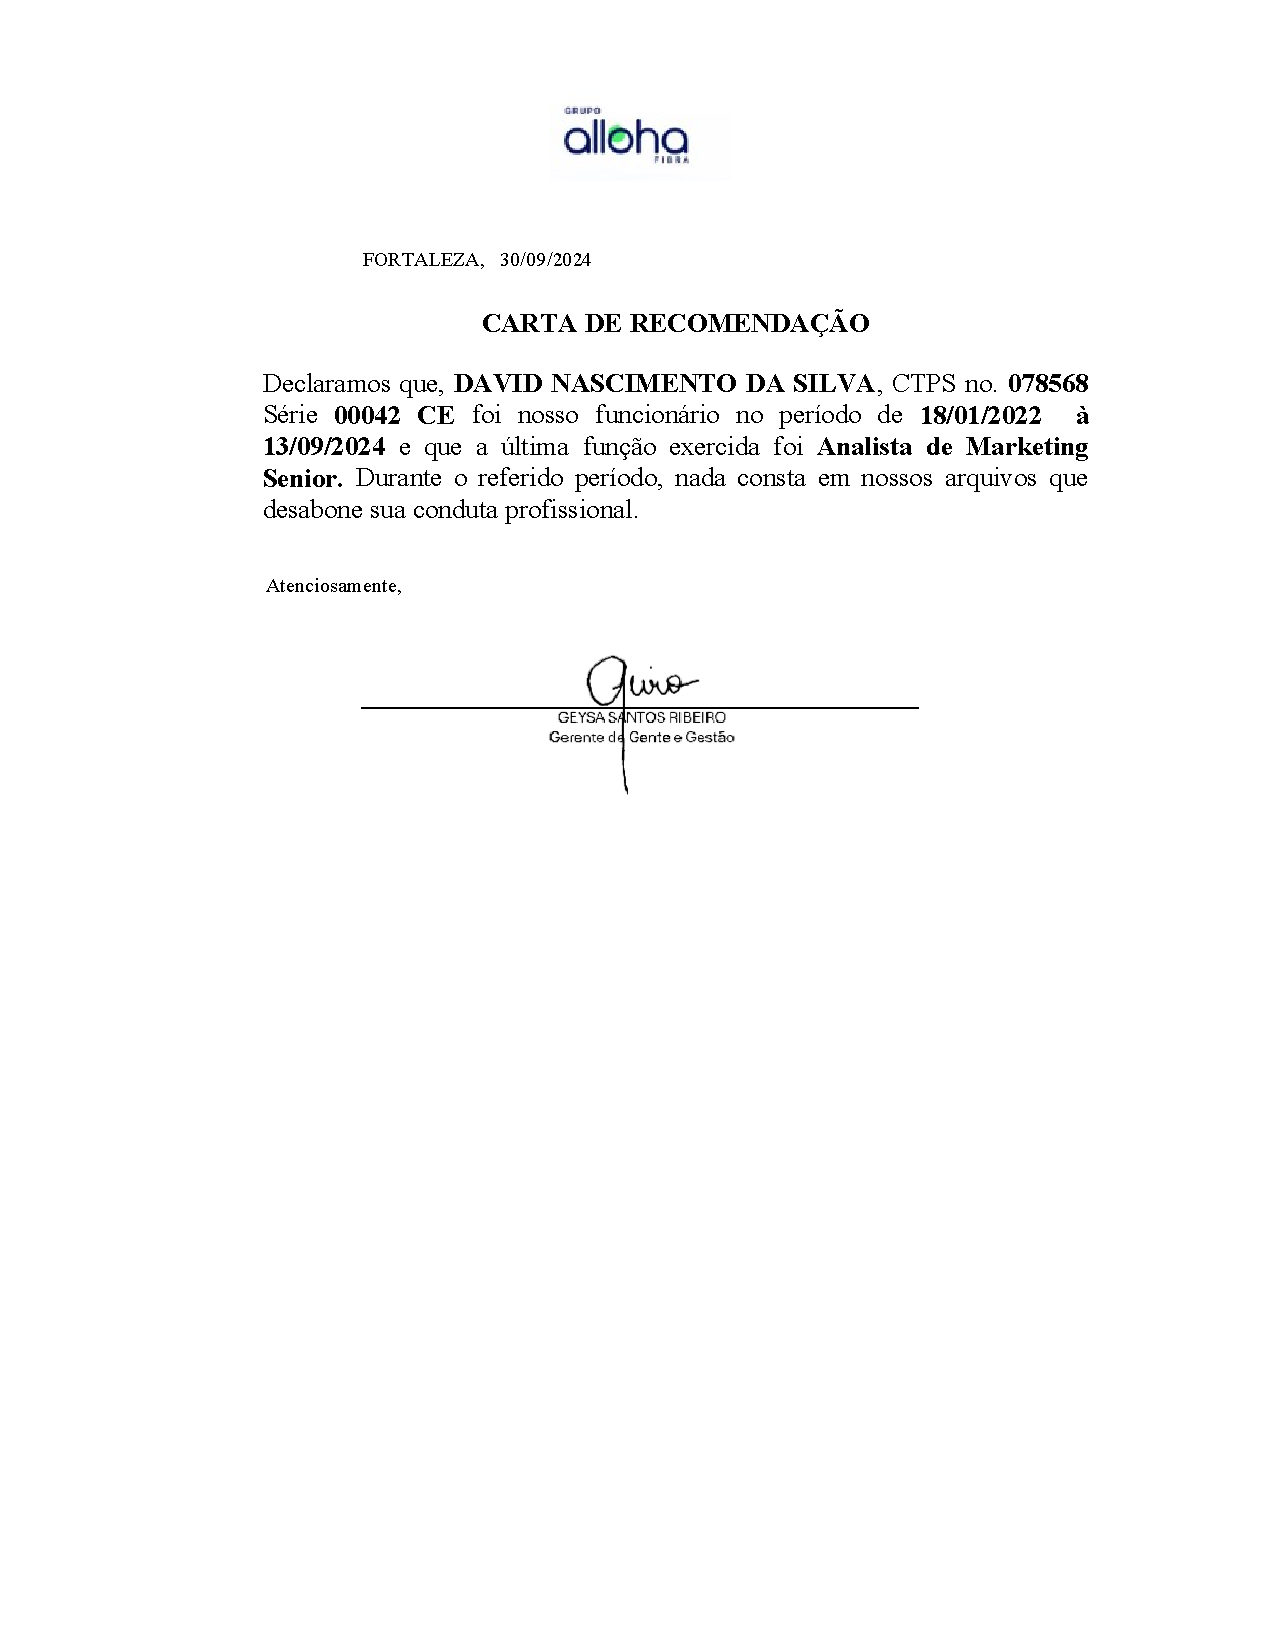
\includegraphics[scale=0.95]{Carta Alloha.pdf}\\
\end{paracol}

%------------------------------------------------------------------------------------------
% Start a 1-column paracol.
\begin{paracol}{1}
	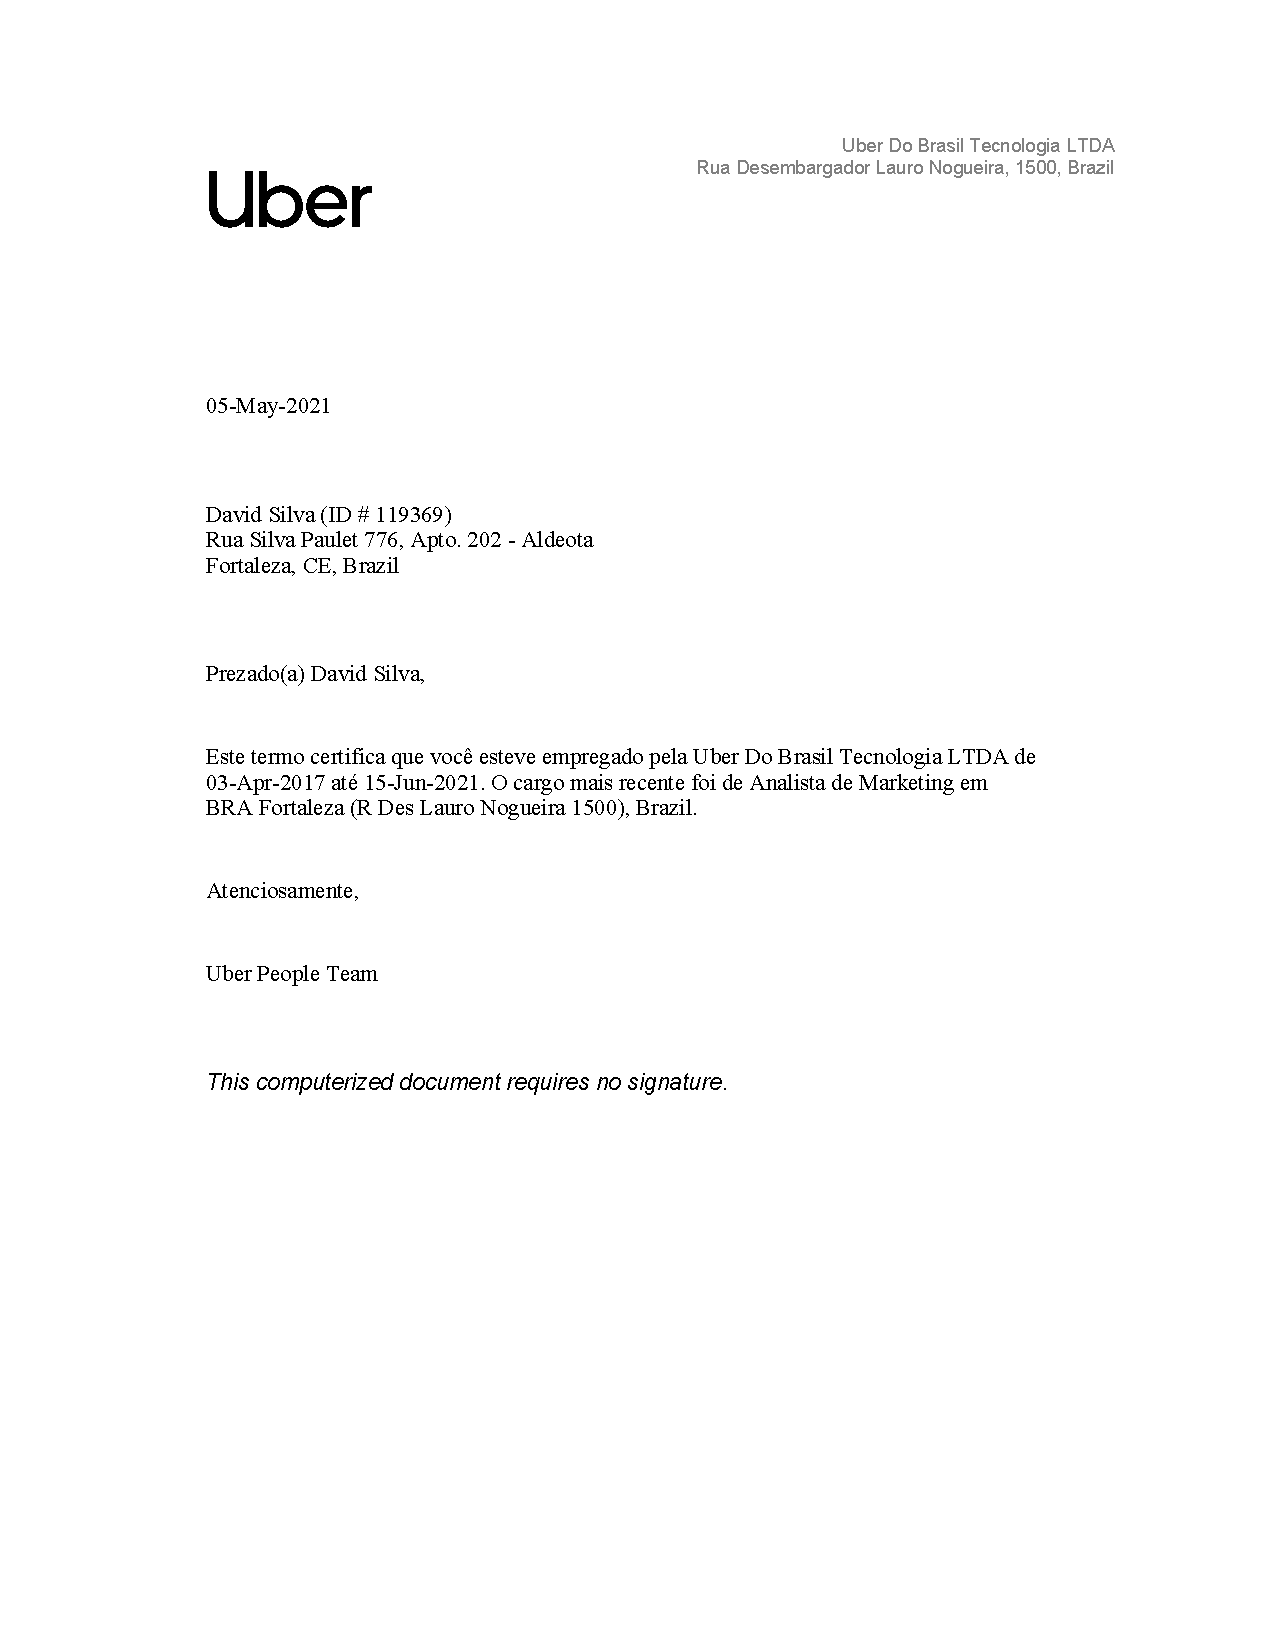
\includegraphics[scale=0.95]{/home/dns/Downloads/Analista_de_Marketing/Conteúdo/Imagem/Carta de recomendaçãoF.pdf}\\
\end{paracol}
%------------------------------------------------------------------------------------------

% use ONLY \newpage if you want to force a page break for
% ONLY the currentc column
%\newpage
%% Set the left/right column width ratio to 1:0.
%\columnratio{1.0}

\end{document}
